\section{Results of the Computational Study}\label{sec:results}

We want to compare the different predictors that we introduced in the last section.
As a metric for the performance of the different predictors, we monitor their average travel times in an $\varepsilon$-DPE with multiple predictors used side by side:
Let $i$ be a commodity with net inflow rate
\[
    u_i(\theta) \coloneqq \begin{cases}
        \bar{u}_i, &\text{ for $\theta \leq h$,}\\
        0, &\text{ for $\theta > h$,}
    \end{cases}
\]
where $\bar{u}_i\in\R_{>0}$ is the constant inflow rate up to some time $h$. 
We denote the outflow rate of commodity $i$ out of the network by  $o_i(\theta) \coloneqq \sum_{e\in\inEdges{t}} f_{i,e}^-(\theta) - \sum_{e\in\outEdges{t}} f_{i,e}^+(\theta)$.
Taking the integral of $u_i(\psi) - o_i(\psi)$ over $[0, \phi]$ yields the amount of flow of commodity $i$ that is inside the network at time $\phi$.
If we integrate the flow inside the network over some time period $[0, H]$ with $H \geq h$, we obtain the \emph{total travel time} of particles of commodity $i$ up to time $H$:
\begin{align*}
    T^{\text{total}}_i
    &\coloneqq\int_0^H \int_0^\phi u_i(\psi) - o_{i}(\psi) \diff\psi \diff \phi.
\end{align*}
The \emph{average travel time} is defined as $T^{\text{avg}}_i\coloneqq  T_i^{\text{total}} / (h\cdot \bar{u}_i)$.

To determine a commodity's regret of a chosen predictor, we additionally need to compute the minimum travel time given a computed $\varepsilon$-DPE $f$.
We first determine the labels $(l_{i,v}(\emptyArg))_{v\in V_i}$ using the Bellman-Ford-Algorithm~\ref{alg:dynamic-bellman-ford} with the dynamic edge costs induced by the computed queue length functions $(q_e(\emptyArg))_{e\in E}$ of $f$.
The minimum travel time at time $\theta$ (up to time horizon $H$) can then be computed using $\min\{H, l_{i,s}(\theta)\} - \theta$.
The \emph{total minimum travel time} of all particles of a commodity can be expressed as
\[
    T^{\mathrm{total}}_{i, \text{OPT}}
    \coloneqq \int_0^H u_i(\theta)\cdot (\min\{H, l_{i,s}(\theta)\} - \theta) \diff \theta
    = \bar u_i \cdot \int_0^h \min\{H, l_{i,s}(\theta)\} - \theta \diff \theta.
\]
From that we derive the \emph{average minimum travel time} as
\[
    T^{\mathrm{avg}}_{i, \text{OPT}}
    \coloneqq \frac{T^{\mathrm{total}}_{i, \text{OPT}}}{\int_0^h u_i(\theta)\diff \theta} = \frac{1}{h}\cdot \int_0^h \min\{H, l_{i,s}(\theta)\} - \theta \diff \theta.
\]

\subsection{Data}

We conduct our experiments on three graphs.
The first is a warm-up synthetic graph with $4$ nodes and $5$ edges. We present the graph in Figure~\ref{fig:synthetic-network}.
The second graph is the road map of Sioux Falls as given in~\cite{LeBlanc1975} which is commonly used in the transport science literature.
This public data set comes with edge attributes free-flow travel time $\tau_e$ and capacity $\nu_e$. 
The third graph is the center of Tokyo, as obtained from Open Street Maps~\cite{openstreetmaps}. 
This graph includes information about the free-flow speed, the length and the numbers of lanes of each road segment $e$.
We compute the transit time $\tau_e$ as the product of the free-flow speed and the length of edge $e$.
The capacity $\nu_e$ is calculated by multiplying the number of lanes with the free-flow speed.

\begin{figure}
    \centering
    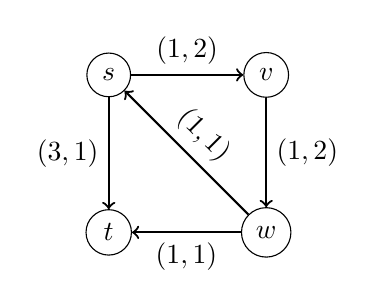
\begin{tikzpicture}
        \node[draw,circle](0)at(0,0) {$s$};
        \node[draw,circle](1)at(2,0) {$v$};
        \node[draw,circle](2)at(0,-2) {$t$};
        \node[draw,circle](3)at(2,-2) {$w$};
        
        \draw[thick,->](0) --node[above]{$(1,2)$} (1);
        \draw[thick,->](1) --node[right]{$(1,2)$} (3);
        \draw[thick,->](3) --node[below]{$(1,1)$} (2);
        \draw[thick,->](3) --node[above,sloped]{$(1,1)$} (0);
        \draw[thick,->](0) --node[left]{$(3,1)$} (2);
    \end{tikzpicture}
    \caption{A network with source $s$ and sink $t$. Edges are labeled with $(\tau_e, \nu_e)$.}\label{fig:synthetic-network}
\end{figure}

In the first network, we only have one commodity with source $s$ and sink $t$ for each predictor. 
For the latter two networks, commodities are randomly chosen.
More detailed information on all networks are depicted in Table~\ref{table:network-data}.
Besides the configuration of all predictors, the average time for computing a single $\varepsilon$-DPE up to time $H$ is shown in row $T^{\mathrm{avg}}_{\mathrm{comp}}$.
Here, each predictor is used by exactly one commodity except for the constant predictor which is used by all other commodities.
The resulting computation times were taken on a single core of an Intel\textsuperscript{\textregistered} Core\textsuperscript{\texttrademark} i7-3520M CPU at $2{.}90$GHz.

\begin{table}[h]
    \centering
    \begin{tabular}{c c c c}
        \textbf{Network} & \textbf{Synthetic} & \textbf{Sioux Falls} & \textbf{Tokyo}
        \\
        \hline
        $\abs{E}$ & $5$ & $75$ &  $4{,}803$
        \\
        $\abs{V}$ & $4$ & $24$ & $3{,}538$
        \\
        $\abs{I}$ & $5$ & $17$ & $40$
        \\
        $[\nu_{\min}, \nu_{\max}]$ & $[1,2]$ & $[4823,25901]$ & $[8, 250]$
        \\
        $[\tau_{\min},\tau_{\max}]$ & $[1,3]$ & $[2, 10]$ & $[0.01, 6.6]$
        \\
        $H$ & $100$ & $100$ & $100$
        \\
        $h$ & $25$ & $25$ & $25$
        \\
        $\varepsilon$ & $0{.}25$ & $1$ & $2{.}5$
        \\
        $H$ for $\predq^\predL$ & $10$ & $20$ & $20$
        \\
        $\delta,H$ for $\predq^\predRL$ & $5,10$ & $1,20$ & $1,20$
        \\
        $\delta,k_p,k_f$ for $\predq^\predML$ & $1,10,10$ & $1,20,20$ & $1,20,20$
        \\
        ML model for $\predq^\predML$ & single & per-edge & single
        \\
        $T^{\mathrm{avg}}_{\mathrm{comp}}$ & $0{.}33s$ & $10{.}92s$ & $343{.}93s$
    \end{tabular}
    \caption{Attributes and configuration of the considered networks.}
    \label{table:network-data}
\end{table}

\subsection{Comparison of Predictors}\label{subsec:comparison-predictors}

In this section we finally carry out the experiments and compare the average travel times of the different predictors.

\subsubsection*{Results on the Synthetic Network}

We first take a closer look at the synthetic network as shown in Figure~\ref{fig:synthetic-network}.
Here, we want to analyze how the average travel times of competing predictors evolve while increasing the total network inflow. 
For each oblivious predictor described in Section~\ref{sec:applied-predictors}, we add a commodity $i\in\{\predq^\predZ, \predq^\predC, \predq^\predL, \predq^\predRL, \predq^\predML \}$.
Each of these commodities has the same source $s$ and sink $t$ and the same constant inflow $\bar u_i$ up to time $h=25$.
The outcome of running the simulation with time horizon $H=100$ for each sampled total inflow in $(0, 30)$ can be seen in Figure~\ref{fig:synthetic-travel-times}.
The ML based predictor performed best, while notably the Zero-Predictor, which distributes flow along paths $(s,t)$ and $(s,v,w,t)$ uniformly at all times, performs better than the remaining predictors.
We note, that here the machine-learned model of the Tokyo network was used.

\begin{figure}[hb]
    \centering
    \input{sample-graph-travel-times}
    \caption{Measured average travel times of competing predictors in the synthetic network in Figure~\ref{fig:synthetic-network}.}\label{fig:synthetic-travel-times}
\end{figure}



\subsubsection*{Results on the Sioux Falls Network}

For the road-networks of Sioux Falls and Tokyo, we randomly generate inflow rates according to the edge capacities of the network.
For each commodity $i$, we ran the simulation after adding $5$ additional commodities with the same source and sink as $i$, one for each predictor, with a very small constant inflow rate.
We monitored their average travel time as a measure of the performance of the different predictors.
All other commodities in the network were assigned the constant predictor, such that the resulting queues should behave similar to the training data.

As the number of edges is small enough in the Sioux Falls network, we trained a separate model for each edge each with a $90\% / 10\%$ split for the training data and test data.
The coefficient of determination was above $0{.}9$ for all edges except for $6$ edges but always higher than $0{.}5$.

Evaluating the average travel time of the different predictors for $12$ random commodities yields the results depicted in Figure~\ref{fig:sioux-falls-boxplot}.
We can see that the linear regression predictor $\predq^\predML$ performs similarly well as the regularized linear predictor $\predq^\predRL$ which is slightly beaten by the constant and the linear predictors.
The Zero predictor performs worse than the others many times.


\begin{figure}[ht]
    \centering
    \begin{tikzpicture}
    \newcommand{\tikzplotwidth}{.5\textwidth}
            \begin{axis}
      [
      width=\tikzplotwidth,
      boxplot/draw direction = y,
      ylabel = {$T_i^{\mathrm{avg}} / T^{\mathrm{avg}}_{\text{OPT}}$},
      xtick = {1, 2, 3, 4, 5},
      xticklabels = {$\hat q^{\text{Z}}$,$\hat q^{\text{C}}$,$\hat q^{\text{L}}$,$\hat q^{\text{RL}}$,$\hat q^{\text{ML}}$},
      every axis plot/.append style = {fill, fill opacity = .1},
      ]
        \addplot + [
              mark = *,
              boxplot,
              color=blue]
              table [row sep = \\, y index = 0] {
            data \\
            0.9999999999999991\\
    1.092389206299255\\
    1.390665342200028\\
    1.259123658488465\\
    1.9412113390756232\\
    1.0766728574729474\\
    1.0000000000000002\\
    1.000309215008037\\
    0.9999999999984845\\
    1.532774006058237\\
    };
    \addplot + [
              mark = *,
              boxplot,
              color=red]
              table [row sep = \\, y index = 0] {
            data \\
            0.9999999999999991\\
    1.1147989787424133\\
    1.1998862431483293\\
    1.015911744853488\\
    1.0541213498029243\\
    1.082240884553064\\
    1.0000000000000002\\
    1.000309215008037\\
    0.9999999999984845\\
    1.0066264386695922\\
    };
    \addplot + [
              mark = *,
              boxplot,
              color={rgb,255:red,0; green,128; blue,0}]
              table [row sep = \\, y index = 0] {
            data \\
            0.9999999999999991\\
    1.159146662968506\\
    1.1769785744216978\\
    1.0434153370332573\\
    1.1101799544732103\\
    1.059710332529087\\
    1.0000000000000002\\
    1.000309215008037\\
    1.0417538653033367\\
    1.0066264386695922\\
    };
    \addplot + [
              mark = *,
              boxplot,
              color=orange]
              table [row sep = \\, y index = 0] {
            data \\
            1.1623605751936434\\
    1.265070792766257\\
    1.165083201559507\\
    1.094305479965723\\
    1.1414866878850014\\
    1.1642709473656274\\
    1.0156019255576745\\
    1.000309215008037\\
    1.0417538653033367\\
    1.361219582558865\\
    };
    \addplot + [
              mark = *,
              boxplot,
              color=black]
              table [row sep = \\, y index = 0] {
            data \\
            0.9999999999999991\\
    1.2086802805809786\\
    1.191841280449055\\
    1.0539407312804374\\
    1.8068753546239809\\
    1.0766728574729474\\
    1.750486457535926\\
    1.1612647695506801\\
    0.9999999999984845\\
    1.0381907210880874\\
    };
    \end{axis}
        \end{tikzpicture}
        
    \caption{Average travel times compared to the minimum average travel time in the Sioux Falls network.}
    \label{fig:sioux-falls-boxplot}
\end{figure}



\subsubsection*{Results on the Tokyo Network}

Because the Tokyo instance has substantially more edges, we decided to train a single model used for all edges.
A training and validation split of $90\%/10\%$ yields a coefficient of determination of $0{.}97$.
Running the evaluation now on $35$ randomly chosen commodities gives the results shown in~\ref{fig:tokyo-boxplot}.
In this scenario, the linear regression predictor performed similarly well as the linear and the constant predictor.
Here, the Zero predictor performs slightly better than the regularized linear predictor, but worse than the remaining three.


\begin{figure}[ht]
    \centering
    \begin{tikzpicture}
        \newcommand{\tikzplotwidth}{.7\textwidth}
    
            \begin{axis}
      [
      width=\tikzplotwidth,
      boxplot/draw direction = y,
      ylabel = {$T_i^{\mathrm{avg}} / T^{\mathrm{avg}}_{\text{OPT}}$},
      xtick = {1, 2, 3, 4, 5},
      xticklabels = {$\hat q^{\text{Z}}$,$\hat q^{\text{C}}$,$\hat q^{\text{L}}$,$\hat q^{\text{RL}}$,$\hat q^{\text{ML}}$},
      every axis plot/.append style = {fill, fill opacity = .1},
      ]
        \addplot + [
              mark = *,
              boxplot,
              color=blue]
              table [row sep = \\, y index = 0] {
            data \\
            1.0035588618990825\\
    1.006875021207046\\
    1.0546632908480962\\
    1.0021185300599227\\
    1.130477139148151\\
    1.000000000000004\\
    1.074361269272079\\
    1.0000394015416956\\
    1.038899346143915\\
    1.4659868432325274\\
    2.281020111570703\\
    1.0187807955718493\\
    1.0324772501539479\\
    1.1747488537469093\\
    1.075830962124691\\
    1.135654990853652\\
    1.0273305442864635\\
    1.1594662519012753\\
    1.005631311302301\\
    1.0000000000000062\\
    1.1420746671031663\\
    1.2922864352775658\\
    1.2519543180188386\\
    1.0309856831865103\\
    1.0250813306566922\\
    1.0268040354819734\\
    1.0000000000000064\\
    1.0249567292206363\\
    1.1218587518906271\\
    };
    \addplot + [
              mark = *,
              boxplot,
              color=red]
              table [row sep = \\, y index = 0] {
            data \\
            1.000939611083866\\
    1.0099965635946615\\
    1.1194191392433437\\
    1.0438303448145665\\
    1.031897468648483\\
    1.000000000000004\\
    1.0275256673183908\\
    1.0001318481019505\\
    1.0661097580719099\\
    1.1395072723569166\\
    1.0773986985703305\\
    1.0296812739241283\\
    1.0543316028453884\\
    1.127207658777134\\
    1.0823477831950046\\
    1.0943328789132778\\
    1.026820605328693\\
    1.04112182308615\\
    1.0104832077734605\\
    1.0000000000000062\\
    1.0001924515887017\\
    1.1090419645074616\\
    1.0559823620866824\\
    1.0484129120989292\\
    1.0250813306566922\\
    1.0268474642986198\\
    1.0000000000000064\\
    1.0253764356096435\\
    1.0928801051591757\\
    };
    \addplot + [
              mark = *,
              boxplot,
              color={rgb,255:red,0; green,128; blue,0}]
              table [row sep = \\, y index = 0] {
            data \\
            1.0015242764529662\\
    1.0099965635946615\\
    1.11599316867238\\
    1.1558483732644247\\
    1.023817281433068\\
    1.0125932960526622\\
    1.0248902488916645\\
    1.0001318481019505\\
    1.0661097580719099\\
    1.1228498319297928\\
    1.0771727270798048\\
    1.0575463447889615\\
    1.0613903185797808\\
    1.1076752947023691\\
    1.0752596852677672\\
    1.0839687021609066\\
    1.024952949662753\\
    1.04112182308615\\
    1.0128168177541301\\
    1.0000000000000062\\
    1.0080386847187672\\
    1.1189974584376732\\
    1.0606205469982737\\
    1.0424589761561809\\
    1.0264370232911584\\
    1.0277036739813534\\
    1.0000000000000064\\
    1.0201179341180944\\
    1.047499003777408\\
    };
    \addplot + [
              mark = *,
              boxplot,
              color=orange]
              table [row sep = \\, y index = 0] {
            data \\
            1.0014772594052734\\
    1.010019091258251\\
    1.251655094217031\\
    1.2945095416359136\\
    1.0524716536104823\\
    1.1417851363471891\\
    1.0486036040011153\\
    1.0001318481019505\\
    1.1697152421776593\\
    1.1373876214069483\\
    1.0912787971417677\\
    1.164336715632529\\
    1.092601393592967\\
    1.116987286919584\\
    1.203865201765564\\
    1.108282997644715\\
    1.0353917309476413\\
    1.04112182308615\\
    1.0203061109904599\\
    1.460736093127774\\
    1.0080386847187672\\
    1.2626083436085247\\
    1.3335136313499878\\
    1.2533047768845929\\
    1.0264370232911584\\
    1.1073458305856372\\
    1.0064472190572746\\
    1.0588292554372767\\
    1.1207559376299927\\
    };
    \addplot + [
              mark = *,
              boxplot,
              color=black]
              table [row sep = \\, y index = 0] {
            data \\
            1.0008767119161566\\
    1.0101929005725585\\
    1.0998771051618013\\
    1.029402147316788\\
    1.0227857757470984\\
    1.000000000000004\\
    1.0275256673183908\\
    1.0001318481019505\\
    1.0661097580719099\\
    1.1707538435334053\\
    1.0791698134047303\\
    1.0296902055933745\\
    1.046954182638017\\
    1.1382076831235102\\
    1.09069836550533\\
    1.1032153662208892\\
    1.0227879112340985\\
    1.04112182308615\\
    1.0104832077734605\\
    1.0000000000000062\\
    1.0006180619467666\\
    1.1088720981468752\\
    1.0575179722199772\\
    1.047305906155529\\
    1.0250813306566922\\
    1.0268474642986198\\
    1.0000000000000064\\
    1.0376540510101842\\
    1.080620525218831\\
    };
    \end{axis}
        \end{tikzpicture}
        
    \caption{Average travel times compared to the minimum average travel time in the Tokyo network.}
    \label{fig:tokyo-boxplot}
\end{figure}
